\documentclass[english,serif,mathserif,xcolor=pdftex,dvipsnames,table]{beamer}
\usetheme{gc3}

\usepackage[T1]{fontenc}
\usepackage[utf8]{inputenc}
\usepackage{babel}

\usepackage{gc3}

\title[Introduction]{%
  GC3Pie basics
}
\author[R. Murri, S3IT UZH]{%
  Riccardo Murri \texttt{<riccardo.murri@uzh.ch>}
  \\[1ex]
  \emph{S3IT: Services and Support for Science IT}
  \\[1ex]
  University of Zurich
}
\date{July~11--14, 2016}

\begin{document}

% title frame
\maketitle

\section{Concepts and glossary}
\part{Concepts and glossary}

\begin{frame}
\frametitle{Parts of GC3Pie}

  GC3Pie consists of three main components:

  \begin{block}{GC3Libs:} Python library for controlling the life-cycle of computational job collections. \end{block}
  \begin{block}{GC3Utils:} This is a small set of low-level utilities exposing the main functionality provided by GC3Libs. \end{block}
  \begin{block}{GC3Apps:} A collection of driver scripts to run large job campaigns. \end{block}
\end{frame}

\begin{frame}
  \frametitle{GC3Pie glossary: Application}
  \begin{quote}
    GC3Pie runs \alert<2-3>{user applications}
    \\
    on clusters and IaaS cloud resources
  \end{quote}

  \uncover<2-3>{
    \+ \alert<2>{An \texttt{Application} is just a command to execute.}

    \+
    \only<2>{If you can run it in the terminal, \\ you can run it in GC3Pie.}
    \only<3>{
      \alert<3>{A single execution of an \texttt{Application} \\ is indeed called a \texttt{Run}.}

      \+ (Other systems might call this a ``job''.)
    }
  }
\end{frame}


\begin{frame}
  \frametitle{GC3Pie glossary: Task}
  \begin{quote}
    GC3Pie \alert{runs} user applications
    \\
    on clusters and IaaS cloud resources
  \end{quote}

  \+ More generally, GC3Pie runs \texttt{Task}s.

  \+ \texttt{Task}s are a superset of applications,
  \\ in that they include workflows.

  %\+ \hyperlink{workflows}{\beamergotobutton{More on this later!}}
\end{frame}


\begin{frame}
  \frametitle{GC3Pie glossary: Resources}
  \begin{quote}
    GC3Pie runs user applications
    \\
    on clusters and IaaS cloud \alert{resources}
  \end{quote}

  \+ \alert{\texttt{Resource}s are the computing infrastructures \\ where GC3Pie executes applications.}

  \+ Resources include: your laptop, the ``Hydra'' cluster, the Science Cloud, Amazon AWS.
\end{frame}


\section{Scaffolding}
\part{Workflow scaffolding}

\begin{frame}[fragile]
  \frametitle{Let's start coding!}
  \begin{columns}
    \begin{column}{0.7\linewidth}
\begin{python}
from gc3libs.cmdline \
  import SessionBasedScript

if __name__ == '__main__':
  import ex2a
  ex2a.AScript().run()

class AScript(SessionBasedScript):
  """
  Minimal workflow scaffolding.
  """
  def __init__(self):
    super(AScript, self).__init__(
        version='1.0')
  def new_tasks(self, extra):
    return []
\end{python}
    \end{column}
    \begin{column}{0.3\linewidth}
      \href{https://raw.githubusercontent.com/uzh/gc3pie/training-july-2016/docs/programmers/tutorials/workflows/solutions/ex2a.py}{Download} this code into a file named \texttt{ex2a.py}

      \+
      Open it in your favorite text editor.
    \end{column}
  \end{columns}
\end{frame}


\begin{frame}[fragile]
  \begin{exercise*}[2.A]

    \+
    \href{https://raw.githubusercontent.com/uzh/gc3pie/training-july-2016/docs/programmers/tutorials/workflows/solutions/ex2a.py}{Download this code} into a file named \texttt{ex2a.py}

    \begin{enumerate}
    \item Run the following command:
\begin{sh}
$ python ex2a.py --help
\end{sh}%$
        Where does the program description in the help text come from?
        Is there anything weird in other parts of the help text?

    \item Run the following command:
\begin{sh}
$ python ex2a.py
\end{sh}%$
        What happens?
      \end{enumerate}
  \end{exercise*}
\end{frame}


\begin{frame}[fragile]
  \begin{columns}[t]
    \begin{column}{0.7\linewidth}
\begin{python}
from gc3libs.cmdline \
  import SessionBasedScript

~\HL{if \_\_name\_\_ == '\_\_main\_\_':}~
  ~\HL{import ex2a}~
  ~\HL{ex2a.AScript().run()}~

class AScript(SessionBasedScript):
  """
  Minimal workflow scaffolding.
  """
  def __init__(self):
    super(AScript, self).__init__(
        version='1.0')
  def new_tasks(self, extra):
    return []
\end{python}
    \end{column}
    \begin{column}{0.4\linewidth}
      \begin{flushright}
        These lines are needed in every session-based script.

        \+
        See \href{https://github.com/uzh/gc3pie/issues/95}{issue 95} for details.
      \end{flushright}
    \end{column}
  \end{columns}
\end{frame}


\begin{frame}[fragile]
  \begin{columns}[t]
    \begin{column}{0.7\linewidth}
\begin{python}
from gc3libs.cmdline \
  import SessionBasedScript

if __name__ == '__main__':
  import ~\HL{ex2a}~
  ~\HL{ex2a}~.AScript().run()

class AScript(SessionBasedScript):
  """
  Minimal workflow scaffolding.
  """
  def __init__(self):
    super(AScript, self).__init__(
        version='1.0')
  def new_tasks(self, extra):
    return []
\end{python}
    \end{column}
    \begin{column}{0.4\linewidth}
      \begin{flushright}
        For this to work, it is \textbf{needed} that this is the
        actual file name.
      \end{flushright}
    \end{column}
  \end{columns}
\end{frame}


\begin{frame}[fragile]
  \begin{columns}
    \begin{column}{0.7\linewidth}
\begin{python}
from gc3libs.cmdline \
  import SessionBasedScript

if __name__ == '__main__':
  import ex2a
  ex2a.AScript().run()

class AScript(SessionBasedScript):
  """
  ~\HL{Minimal workflow scaffolding.}~
  """
  def __init__(self):
    super(AScript, self).__init__(
        version='1.0')
  def new_tasks(self, extra):
    return []
\end{python}
    \end{column}
    \begin{column}{0.4\linewidth}
      \begin{flushright}
        This is the \\ program's help text!
      \end{flushright}
    \end{column}
  \end{columns}
\end{frame}


\begin{frame}[fragile]
  \begin{columns}
    \begin{column}{0.7\linewidth}
\begin{python}
from gc3libs.cmdline \
  import SessionBasedScript

if __name__ == '__main__':
  import ex2a
  ex2a.AScript().run()

class AScript(SessionBasedScript):
  """
  Minimal workflow scaffolding.
  """
  def __init__(self):
    super(AScript, self).__init__(
      ~\HL{version='1.0'}~)
  def new_tasks(self, extra):
    return []
\end{python}
    \end{column}
    \begin{column}{0.4\linewidth}
      \begin{flushright}
        A version number \\ is \textbf{mandatory}.
      \end{flushright}
    \end{column}
  \end{columns}
\end{frame}


\begin{frame}[fragile]
  \begin{columns}
    \begin{column}{0.7\linewidth}
\begin{python}
from gc3libs.cmdline \
  import SessionBasedScript

if __name__ == '__main__':
  import ex2a
  ex2a.AScript().run()

class AScript(SessionBasedScript):
  """
  Minimal workflow scaffolding.
  """
  def __init__(self):
    super(AScript, self).__init__(
        version='1.0')
  def new_tasks(self, extra):
    ~\HL{return []}~
\end{python}
    \end{column}
    \begin{column}{0.4\linewidth}
      \begin{flushright}
        \textbf{This is the core of the script.}

        \+
        Return a list of \texttt{Application} objects, that GC3Pie will execute.
      \end{flushright}
    \end{column}
  \end{columns}
\end{frame}


\section{Applications}
\part{The \texttt{Application} object}

\begin{frame}
  \frametitle{Specifying commands to run, I}

  You need to ``describe'' an application to GC3Pie, in order for
  GC3Pie to use it.

  \+
  This ``description'' is a blueprint from which many actual
  command instances can be created.

  \+
  (A few such ``descriptions'' are already part of the core library.)
\end{frame}


\begin{frame}
  \frametitle{GC3Pie application model}

  In GC3Pie, an application ``description'' is an object of the
  \texttt{gc3libs.Application} class (or subclasses thereof).

  \+
  At a minimum: provide application-specific command-line invocation.

  \+
  Advanced users can customize pre- and post-processing, react on
  state transitions, set computational requirements based on input
  files, influence scheduling.  (This is standard OOP: subclass and
  override a method.)
\end{frame}


\begin{frame}[fragile]
\frametitle{A basic example: grayscaling}
\begin{sh}
$ convert lena.jpg -colorspace gray lena-gray.jpg
\end{sh}%$
\begin{tabular}{ccc}
  {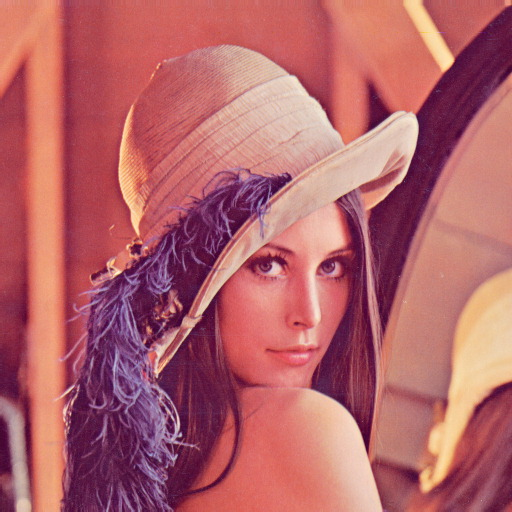
\includegraphics[width=0.4\linewidth]{fig/lena.jpg}}
  &
  {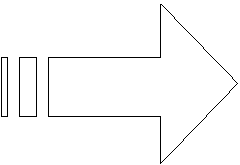
\includegraphics[width=0.1\linewidth,totalheight=0.45\textheight]{fig/arrow.pdf}}
  &
  {\includegraphics[width=0.4\linewidth]{fig/gray-lena.jpg}}
\end{tabular}

\end{frame}


\begin{frame}[fragile]
\frametitle{Grayscaling example, I}

  Here is how you would tell GC3Pie \\ to run that command-line.

\begin{python}
from gc3libs import Application

class GrayscaleApp(Application):
  """Convert an image file to grayscale."""
  def __init__(self, img):
    inp = basename(img)
    out = "gray-" + inp
    Application.__init__(
      self,
      arguments=[
        "convert", inp, "-colorspace", "gray", out],
      inputs=[img],
      outputs=[out],
      output_dir="grayscale.d",
      stdout="stdout.txt")
\end{python}
\end{frame}


\begin{frame}[fragile]
\frametitle{Always inherit from Application}

  Your application class must inherit from class \texttt{gc3libs.Application}
  \+
\begin{python}
~\HL{from gc3libs import Application}~

class GrayscaleApp~\HL{(Application)}~:
  """Convert an image file to grayscale."""
  def __init__(self, img):
    inp = basename(img)
    out = "gray-" + inp
    Application.__init__(
      self,
      arguments=[
        "convert", inp, "-colorspace", "gray", out],
      inputs=[img],
      outputs=[out],
      output_dir="grayscale.d",
      stdout="stdout.txt")
\end{python}
\end{frame}


\begin{frame}[fragile]
  \frametitle{The \texttt{arguments} parameter, I}

  The \texttt{arguments=} parameter is the actual command-line to be invoked.

  \+
\begin{python}
class GrayscaleApp(Application):
  """Convert an image file to grayscale."""
  def __init__(self, img):
    inp = basename(img)
    out = "gray-" + inp
    Application.__init__(
      self,
      ~\HL{arguments=[}~
        ~\HL{"convert", inp, "-colorspace", "gray", out],}~
      inputs=[img],
      outputs=[out],
      output_dir="grayscale.d",
      stdout="stdout.txt")
\end{python}
\end{frame}

\begin{frame}[fragile]
\frametitle{The \texttt{arguments} parameter, II}

The first item in the \texttt{arguments} list is the name or path to the command to run.

  \+
\begin{python}
class GrayscaleApp(Application):
  """Convert an image file to grayscale."""
  def __init__(self, img):
    inp = basename(img)
    out = "gray-" + inp
    Application.__init__(
      self,
      arguments=[
        ~\HL{"convert"}~, inp, "-colorspace", "gray", out],
      inputs=[img],
      outputs=[out],
      output_dir="grayscale.d",
      stdout="stdout.txt")
\end{python}
\end{frame}

\begin{frame}[fragile]
\frametitle{The \texttt{arguments} parameter, III}

The rest of the list are arguments to the program, as you would type
them at the shell prompt.

  \+
\begin{python}
class GrayscaleApp(Application):
  """Convert an image file to grayscale."""
  def __init__(self, img):
    inp = basename(img)
    out = "gray-" + inp
    Application.__init__(
      self,
      arguments=[
        "convert", ~\HL{inp, "-colorspace", "gray", out}~],
      inputs=[img],
      outputs=[out],
      output_dir="grayscale.d",
      stdout="stdout.txt")
\end{python}
\end{frame}


\begin{frame}[fragile]
\frametitle{The \texttt{inputs} parameter, I}

The \texttt{inputs} parameter holds a list of files that you want to
\emph{copy} to the location where the command is executed. (Remember:
this might be a remote computer!)

  \+
\begin{python}
class GrayscaleApp(Application):
  """Convert an image file to grayscale."""
  def __init__(self, img):
    inp = basename(img)
    out = "gray-" + inp
    Application.__init__(
      self,
      arguments=[
        "convert", inp, "-colorspace", "gray", out],
      ~\HL{inputs=[img]}~,
      outputs=[out],
      output_dir="grayscale.d",
      stdout="stdout.txt")
\end{python}
\end{frame}


\begin{frame}[fragile]
  \frametitle{The \texttt{inputs} parameter, II}

  Input files retain their name during the copy, \\ but not the entire path.

  \+
  For example:
  \begin{python}
    inputs = [
      '/home/rmurri/values.dat',
      '/home/rmurri/stats.csv',
    ]
  \end{python}
  will make files \emph{values.dat} and \emph{stats.csv} available in
  the command execution directory.

\end{frame}


\begin{frame}[fragile]
  \frametitle{The \texttt{inputs} parameter, III}

  You need to pass the full path name into the
  \texttt{inputs} list, but use only the ``base name'' in the command
  invocation.

\begin{python}
class GrayscaleApp(Application):
  """Convert an image file to grayscale."""
  def __init__(self, img):
    ~\HL{inp = basename(img)}~
    out = "gray-" + inp
    Application.__init__(
      self,
      arguments=[
        "convert", ~\HL{inp}~, "-colorspace", "gray", out],
      inputs=[~\HL{img}~],
      outputs=[out],
      output_dir="grayscale.d",
      stdout="stdout.txt")
\end{python}
\end{frame}


\begin{frame}[fragile]
\frametitle{The \texttt{outputs} parameter, I}

The \texttt{outputs} argument list files that should be copied from
the command execution directory back to your computer.

  \+
\begin{python}
class GrayscaleApp(Application):
  """Convert an image file to grayscale."""
  def __init__(self, img):
    inp = basename(img)
    out = "gray-" + inp
    Application.__init__(
      self,
      arguments=[
        "convert", inp, "-colorspace", "gray", out],
      inputs=[img],
      ~\HL{outputs=[out]}~,
      output_dir="grayscale.d",
      stdout="stdout.txt")
\end{python}
\end{frame}


\begin{frame}[fragile]
  \frametitle{The \texttt{outputs} parameter, II}

  Output file names are \emph{relative to the execution directory}.
  For example:
  \begin{python}
    outputs = ['result.dat', 'program.log']
  \end{python}

  \+
  (Contrast with input files, which must be specified by
  \emph{absolute path}, e.g., \texttt{/home/rmurri/values.dat})

  \+
  Any file with the given name that is found in the execution
  directory will be copied back. (\emph{Where?} See next slides!)

  \+
  If an output file is \emph{not} found, this is \emph{not} an
  error. In other words, \textbf{output files are optional}.
\end{frame}


\begin{frame}[fragile]
\frametitle{The \texttt{output\_dir} parameter, I}

The \lstinline|output_dir| parameter specifies where output filess
will be downloaded.

\+
\begin{python}
class GrayscaleApp(Application):
  """Convert an image file to grayscale."""
  def __init__(self, img):
    inp = basename(img)
    out = "gray-" + inp
    Application.__init__(
      self,
      arguments=[
        "convert", inp, "-colorspace", "gray", out],
      inputs=[img],
      outputs=[out],
      ~\HL{output\_dir="grayscale.d"}~,
      stdout="stdout.txt")
\end{python}
\end{frame}


\begin{frame}[fragile]
  \frametitle{The \emph{output\_dir} parameter, II}

  By default, GC3Pie does not overwrite an existing output directory:
  it will move the existing one to a backup name.

  \+
  So, if \texttt{grayscale.d} already exists, GC3Pie will:
  \begin{enumerate}
  \item rename it to \lstinline|grayscale.d.~1~|
  \item create a new directory \texttt{grayscale.d}
  \item download output files into the new directory
  \end{enumerate}
\end{frame}


\begin{frame}[fragile]
\frametitle{The \texttt{stdout} parameter}

This specifies that the command's \emph{standard output} should be
saved into a file named \texttt{stdout.txt} and retrieved along with
the other output files.

  \+
\begin{python}
class GrayscaleApp(Application):
  """Convert an image file to grayscale."""
  def __init__(self, img):
    inp = basename(img)
    out = "gray-" + inp
    Application.__init__(
      self,
      arguments=[
        "convert", inp, "-colorspace", "gray", out],
      inputs=[img],
      outputs=[out],
      output_dir="grayscale.d",
      ~\HL{stdout="stdout.txt"}~)
\end{python}
\end{frame}


\begin{frame}[fragile]
\frametitle{(The \texttt{stderr} parameter)}

There's a corresponding \texttt{stderr} option for the command's
\emph{standard error} stream.

\begin{python}
class GrayscaleApp(Application):
  """Convert an image file to grayscale."""
  def __init__(self, img):
    inp = basename(img)
    out = "gray-" + inp
    Application.__init__(
      self,
      arguments=[
        "convert", inp, "-colorspace", "gray", out],
      inputs=[img],
      outputs=[out],
      output_dir="grayscale.d",
      stdout="stdout.txt",
      ~\HL{stderr="stderr.txt"}~)
\end{python}
\end{frame}


\begin{frame}
  \frametitle{Mixing \texttt{stdout} and \texttt{stderr} capture}

  You can specify \textbf{either one} of the \texttt{stdout} and
  \texttt{stderr} parameters, \textbf{or both}.

  \+
  If you give both, and they have the same value, then
  \texttt{stdout} and \texttt{stderr} will be intermixed just as they
  are in normal screen output.
\end{frame}


\begin{frame}[fragile]
  \frametitle{Let's run!}
  In order for a session-based script to execute something, its
  \texttt{new\_tasks()} method must return a list of
  \texttt{Application} objects to run.

\+
\begin{python}
class AScript(SessionBasedScript):
  # ...
  def new_tasks(self, extra):
    # `self.param.args' is the list
    # of command-line arguments
    input_file = self.params.args[0]
    app = GrayscaleApp(input_file)
    return [app]
\end{python}
\end{frame}

\begin{frame}[fragile]
  \small

  \begin{exercise*}[2.B]

    \+
    Edit the \texttt{ex2a.py} file: insert the code to define the
    \href{https://raw.githubusercontent.com/uzh/gc3pie/training-july-2016/docs/programmers/tutorials/workflows/downloads/grayscale_app.py}{\texttt{GrayscaleApp}}
    application, and modify the \texttt{new\_tasks()} method to return
    one instance of it (as in the previous slide).

    \+
    Can you convert the \href{https://raw.githubusercontent.com/uzh/gc3pie/training-july-2016/docs/programmers/tutorials/workflows/lena.jpg}{\texttt{lena.jpg}} file to gray-scale using
    this GC3Pie script?

    \+ \footnotesize
    {\em (You can download the code for \texttt{GrayscaleApp} and the ``Lena'' image file from
    \href{https://raw.githubusercontent.com/uzh/gc3pie/training-july-2016/docs/programmers/tutorials/workflows/}{this
      URL}.)}
  \end{exercise*}

  \+
  \begin{exercise*}[2.C]

    Edit the script from Exercise 2.B above and add the ability to
    convert multiple files: for each file name given on the command
    line, an instance of \texttt{GrayscaleApp} should be run.
  \end{exercise*}
\end{frame}


\section{Resource definition}
\part{Resource definition}

\begin{frame}[fragile]
  \frametitle{The \texttt{gservers} command}

  The \texttt{gservers} command is used to see \alert<2>{configured} and
  available resources.

\+
\begin{stdout}
$ gservers
+---------------------+--------------------------+-----------+
|                     | localhost                |           |
+---------------------+--------------------------+-----------+
|            frontend | ( Frontend host name )   | localhost |
|                type | ( Access mode )          | shellcmd  |
|             updated | ( Accessible? )          | True      |
|              queued | ( Total queued jobs )    | 0         |
|         user_queued | ( Own queued jobs )      | 0         |
|            user_run | ( Own running jobs )     | 6         |
|   max_cores_per_job | ( Max cores per job )    | 4         |
| max_memory_per_core | ( Max memory per core )  | 8GiB      |
|        max_walltime | ( Max walltime per job ) | 8hour     |
+---------------------+--------------------------+-----------+
\end{stdout}%$

\uncover<2>{%
  \small \alert<2>{Resources are defined in file \texttt{\$HOME/.gc3/gc3pie.conf}}
}
\end{frame}


\begin{frame}[fragile,label=resources]
  \frametitle{Example execution resources: local host}
  \begin{columns}[t]
    \begin{column}{0.5\textwidth}
      Allow GC3Pie to run tasks on the local computer.

      \+ This is the default installed by GC3Pie
      into \lstinline|$HOME/.gc3/gc3pie.conf| %$
    \end{column}
    \begin{column}{0.5\textwidth}
  \begin{stdout}
[resource/localhost]
enabled = yes
type = shellcmd
frontend = localhost
transport = local
max_cores_per_job = 2
max_memory_per_core = 2GiB
max_walltime = 8 hours
max_cores = 2
architecture = x86_64
auth = none
override = no
\end{stdout}
    \end{column}
  \end{columns}
\end{frame}


\begin{frame}[fragile]
  \frametitle{Example execution resources: SLURM}
  \begin{columns}[t]
    \begin{column}{0.5\textwidth}
      Allow submission of jobs to the ``Hydra'' cluster.
    \end{column}
    \begin{column}{0.5\textwidth}
\begin{stdout}
[resource/hydra]
enabled = no
type = slurm
frontend = login.s3it.uzh.ch
transport = ssh
auth = ssh_user_rmurri
max_walltime = 1 day
max_cores = 96
max_cores_per_job = 64
max_memory_per_core = 1 TiB
architecture = x86_64
prologue_content =
  module load cluster/largemem

[auth/ssh_user_rmurri]
type=ssh
username=rmurri
\end{stdout}
    \end{column}
  \end{columns}
\end{frame}


\begin{frame}[fragile]
  \frametitle{Example execution resources: OpenStack}
  \begin{columns}[t]
    \begin{column}{0.5\textwidth}
\begin{stdout}
[resource/sciencecloud]
enabled=no
type=openstack+shellcmd
auth=openstack

vm_pool_max_size = 32
security_group_name=default
security_group_rules=
  tcp:22:22:0.0.0.0/0,
  icmp:-1:-1:0.0.0.0/0
network_ids=
  c86b320c-9542-4032-a951-c8a068894cc2

# definition of a single execution VM
instance_type=1cpu-4ram-hpc
image_id=2b227d15-8f6a-42b0-b744-ede52ebe59f7

max_cores_per_job = 8
max_memory_per_core = 4 GiB
max_walltime = 90 days
max_cores = 32
architecture = x86_64

# how to connect
vm_auth=ssh_user_ubuntu
keypair_name=rmurri
public_key=~/.ssh/id_dsa.pub
\end{stdout}
    \end{column}
    \begin{column}{0.5\textwidth}
      \begin{stdout}
[auth/ssh_user_ubuntu]
# default user on Ubuntu VM images
type=ssh
username=ubuntu


[auth/openstack]
# only need to set the `type` here;
# any other value will be taken from
# the `OS\_*` environment variables
type = openstack
      \end{stdout}

      \+\+\+
      Allow running tasks on the ``ScienceCloud'' VM infrastructure.

      % \+ \footnotesize
      % Cloud-based submission happens in two steps:
      % \emph{(1)} create a VM, \emph{(2)} SSH to it and run jobs.  Each
      % step requires different connection and authentication.
    \end{column}
  \end{columns}
\end{frame}


\begin{frame}
  \begin{exercise*}[2.D]
    Change the configuration file
    \texttt{{\textasciitilde}/.gc3/gc3pie.conf} to enable the
    \texttt{sciencecloud} resource.  Verify with the \texttt{gservers}
    command that it works.
  \end{exercise*}

  \+
  \begin{exercise*}[2.E]
    Run the grayscale converter \texttt{ex2c} on Science Cloud.
    Do you need to change anything in the code?
  \end{exercise*}
\end{frame}


\end{document}

%%% Local Variables:
%%% mode: latex
%%% TeX-master: t
%%% End:
